\section{Actividades a Realizar y Orientaciones para su Desarrollo}
Siga estos pasos detallados para instalar GNS3 Server y Client en Rocky Linux 9:

\subsection{Instalar Git}

Para instalar Git, escribe el siguiente comando en la terminal de Rocky Linux 9: 
\begin{terbox} 
sudo dnf install git 
\end{terbox} 

Presiona Enter para confirmar la instalación. Git se instalará en tu sistema.

\subsection{Configurar Git}

Una vez instalado Git, es importante configurarlo para que funcione correctamente. Para hacerlo, escribe los siguientes comandos: 

\begin{terbox} 
git config --global user.name "Your Name"\\
git config --global user.email "your\_email@example.com" 
\end{terbox} 

Reemplaza "Your Name" con tu nombre real o el nombre que deseas utilizar en tus commits y establece la dirección de correo electrónico con tu dirección de correo electrónico real.



\subsection{Conectar al Repositorio GitHub}
Para evitar tener que ingresar tu usuario y contraseña cada vez que haces push o pull, 
es recomendable usar SSH. 
\begin{terbox}
\begin{verbatim}
ssh-keygen -t rsa -b 4096 -C "email@domain.com"
Generating public/private rsa key pair.
...
...
+----[SHA256]-----+

\end{verbatim}
\end{terbox}

Presiona Enter para aceptar la ubicación predeterminada o selecciona una específica y, si lo deseas, añade una frase de contraseña para mayor seguridad. 
Luego accede al archivo de la clave pública creada y copia su contenido.

\begin{terbox}
    \begin{verbatim}
cat ~/.ssh/git_rsa.pub
ssh-rsa...
... 
...
email@domain.com
    \end{verbatim}
    \end{terbox}
    
    En una cuenta creada en GitHub, acceder a la sección de \href{https://github.com/settings/keys}{configuraciónes} para crear añadir una nueva clave de autorización ssh. 
    Completar la información y en la sección key pegar la clave pública copiada de git\_rsa.pub.
\begin{figure}[H]
    \centering
    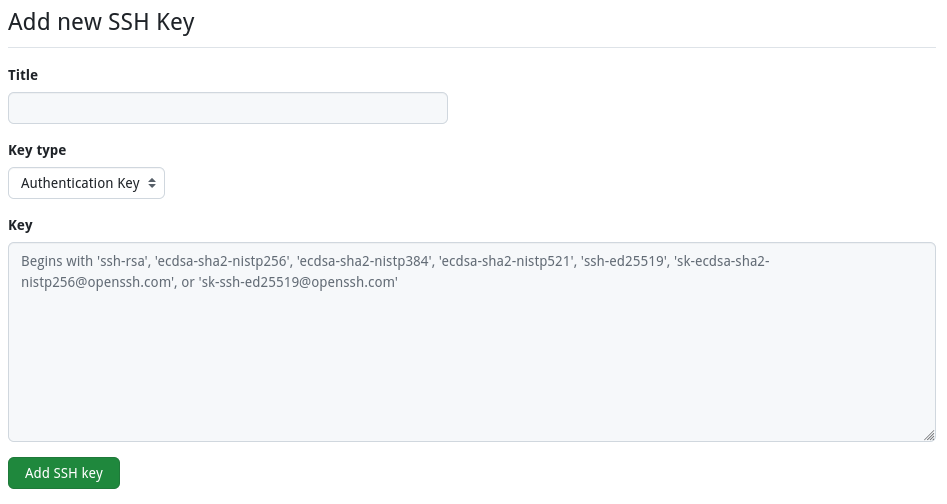
\includegraphics[width=0.8\linewidth]{Imagenes/sshkey.png}
    \caption{Creación de nueva clave ssh para GitHub}
    \label{fig_sshkey}
\end{figure}


Se puede verificar que todo esté configurado correctamente ejecutando el comando:

\begin{terbox}
    \begin{verbatim}
ssh -T git@github.com
...
...
This key is not known by any other names
Are you sure you want to continue connecting (yes/no/[fingerprint])?
Hi fresvel! You've successfully authenticated, but GitHub does not 
provide shell access.
    \end{verbatim}
\end{terbox}

Finalmente crear un nuevo repositorio en \href{https://github.com/new}{GitHub} al que se enlazará el proyecto local

\subsection{Crear un repositorio local}
Para crear un repositorio local, escribe los siguientes comandos

\begin{terbox} 
\begin{verbatim}
mkdir myproject
cd myproject
git init
git add .
git commit -m "Mi primer commit"
git branch -M main 
git remote add origin git@github.com:user/name_repo.git
git push -u origin main
\end{verbatim}
\end{terbox} 

Esto creará un directorio llamado "myproject" y inicializará un repositorio Git dentro de él.




\subsection{Agregar archivos al repositorio}

Para agregar archivos al repositorio, escribe el siguiente comando: \begin{terbox} 
 

\end{terbox} 

Este comando agrega todos los archivos en el directorio actual al staging (área de preparación) para el próximo commit.

\subsection{Realizar el primer commit}

Para realizar el primer commit, escribe el siguiente comando: \begin{terbox} 

\end{terbox}

Este comando crea un commit con el mensaje "Initial commit" y agrega todos los archivos en el staging al repositorio.

\subsection{Conectar con GitHub}

Para conectar con GitHub, necesitarás crear un repositorio en GitHub y obtener la URL del repositorio. Luego, escribe el siguiente comando: 


Reemplaza "your\_username" y "your\_repository\_name" con tus credenciales de GitHub.

\subsection{Enviar el repositorio a GitHub}

Para enviar el repositorio a GitHub, escribe el siguiente comando: \begin{terbox} 
git push -u origin master 
\end{terbox} 

Este comando envía el repositorio a GitHub y crea una rama llamada "master".

\subsection{Verificar el repositorio en GitHub}

Para verificar que el repositorio se haya enviado correctamente a GitHub, abre una ventana de exploración y ve a tu repositorio en GitHub. Deberías ver que el repositorio ha sido creado correctamente y que contiene los archivos que agregaste en el paso 4.




